%Shreyas ugemuge, sr design Design doc source
\documentclass[12pt]{article}

%%Packages
\usepackage{color}
\usepackage{enumitem}
\usepackage{setspace}
\usepackage{tabularx}
%\usepackage{tikz}
%\tikzstyle{class}=[
%    rectangle,
%    draw=black,
%    text centered,
%    anchor=north,
%    text=black,
%    text width=3cm]
\usepackage{authblk}
\usepackage[document]{ragged2e}
\usepackage[left=1in,right=1in,top=1in,bottom=1in]{geometry}
\usepackage{graphicx}
\usepackage[pdftex,pdfpagelabels,bookmarks,hyperindex,hyperfigures]{hyperref}
%%%%%%%

%%Title and author
\title{\textbf{Design Document} \\ \hfill \break
	Academic Behaviour Recommendation system}
	
\author{Shreyas Ugemuge\      \texttt{sugemuge2014@my.fit.edu}
  \and
  Yaqeen AlKathiri\      \texttt{yalkathiri2013@my.fit.edu}
  \and
	Mohammed AlHabsi\      \texttt{malhabsi2013@my.fit.edu}
  \and
  Shiru Hou\      \texttt{shou2015@my.fit.edu}
  \and
  Faculty Sponsor: Dr. Phillip Chan\      \texttt{pkc@cs.fit.edu}}
  
  \date{\today \\ v1.0}

\begin{document}
\maketitle
\pagebreak
\tableofcontents
\pagebreak
\section{Introduction}
This document explores the interface for the system.
\section{Use Case for Student Performance Analysis}
\subsection{Main Success scenario (Student)}
\begin{enumerate}
	\item User opens the program
	\item User Chooses student
	\item User logs on
	\item Use chooses course name
	\item user clicks on get suggestions
	\item Report is displayed
\end{enumerate}
\subsection{Main success scenario (Teacher)}
\begin{enumerate}
	\item user opens the program
	\item user chooses teacher
	\item user logs on
	\item user manually enters data from syllabus
	\item user uploads log and grade file
	\item Report is displayed
 \end{enumerate}
\section{System Sequence Diagram}
\begin{figure}
\caption{Student SSD}

\includegraphics[width=\textwidth]{img/1} 
\end{figure}
\begin{figure}
	\caption{Teacher SSD}

\includegraphics[width=\textwidth]{img/2.png}
\end{figure}
\pagebreak
\section{UML diagrams}
\begin{tabularx}{7cm}{|X|}
	\hline
	ExtractBehaviors \\
	\hline
	\dots \\
	\hline
	+ prepareLogFile(File) : void\\
	+ getBehaviors(File) : Behaviors\\
	+ toString() : String\\
	\dots \\
	\hline
\end{tabularx}
\hfil 
\begin{tabularx}{7cm}{|X|}
	\hline
	ExtractPerformance \\
	\hline
	\dots \\
	\hline
	+ prepareGradeFile(File) : void\\
	+ getPerformance(File) : Behaviors\\
	+ toString() : String \\
	\dots \\
	\hline
\end{tabularx}
\\ \hfill \break
\begin{tabularx}{7cm}{|X|}
	\hline
	CorrelateData \\
	\hline
	\dots \\
	\hline
	+ prepareBehaviors(File) : void\\
	+ getBehaviors(File) : Behaviors\\
	+ prepareGradeFile(File) : void\\
	+ getPerformance(File) : Behaviors\\
	+ toString() : String \\
	\dots \\
	\hline
\end{tabularx}
\pagebreak
\section{Interface Mock ups}

\begin{figure}[h]
	\caption{Welcome screen}
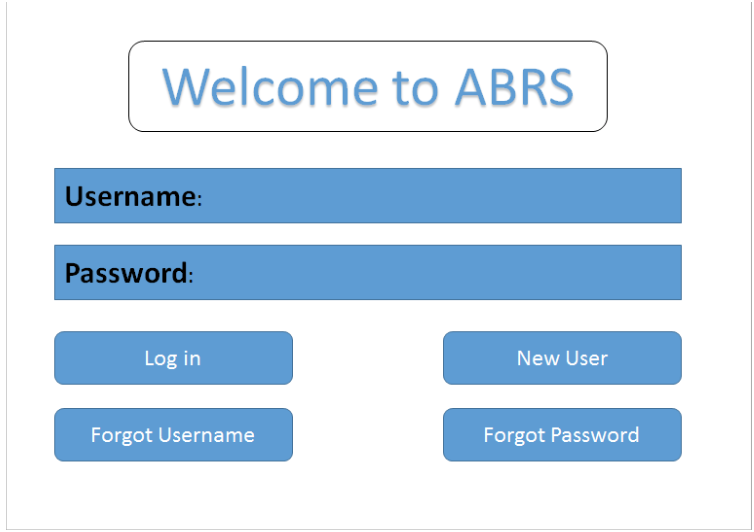
\includegraphics[width=\textwidth]{img/3} 
\end{figure}
\begin{figure}[h]
	\caption{signup screen}
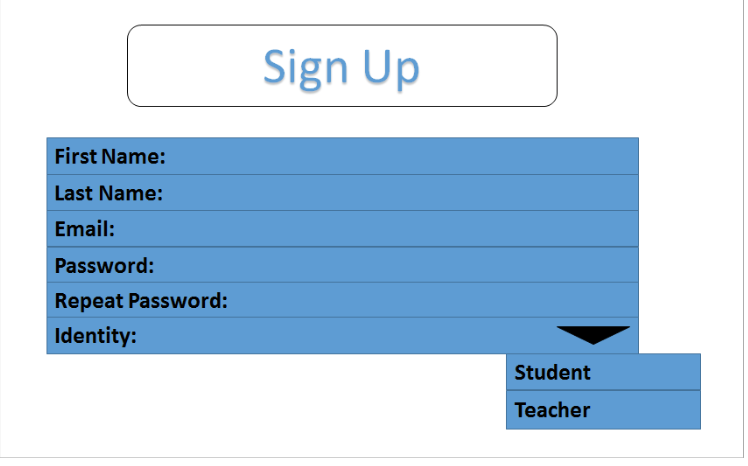
\includegraphics[width=\textwidth]{img/4} 
\end{figure}
\begin{figure}
	\caption{Choose interface screen}

\includegraphics[width=\textwidth]{img/5} 
\end{figure}
\begin{figure}
\caption{Upload}
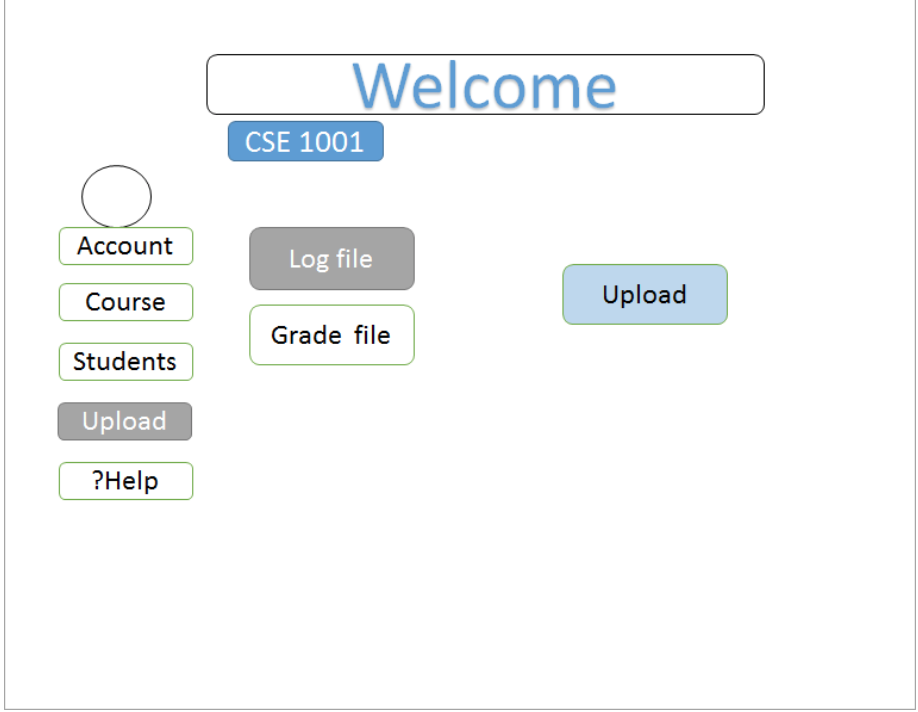
\includegraphics[width=\textwidth]{img/6} 
\end{figure}
\begin{figure}
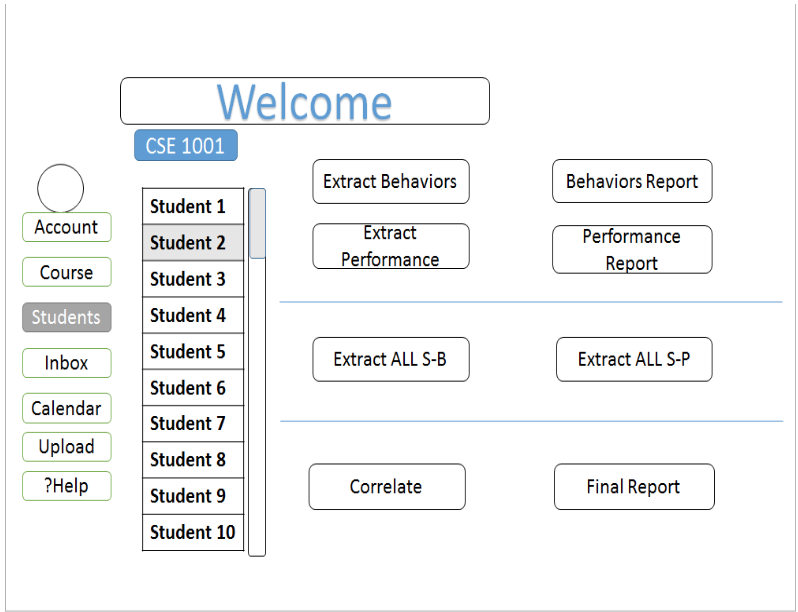
\includegraphics[width=\textwidth]{img/7}
\end{figure}

\begin{figure}
\caption{Report}
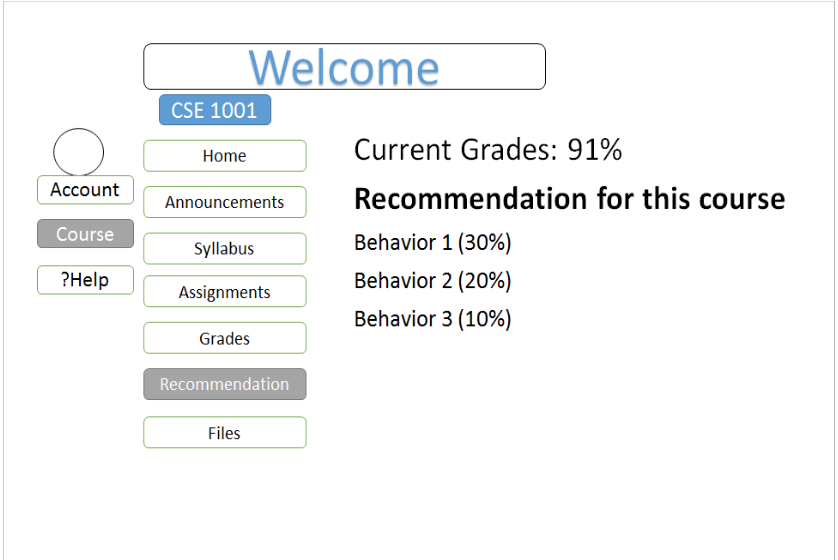
\includegraphics[width=\textwidth]{img/8} 
\end{figure}

\end{document}